\chapter{Materály a metódy}

\section{Ciele}

Cieľom tejto práce je urobiť scientimetrickú analýzu FPV UCM v Trnave.  Tento
cieľ sme rozdelili do nasledujúcich krokov:

\begin{enumerate}

\item Z dvoch najväčších citačných databáz \emph{Thomson Reuters Web of Science}
  a \emph{Scopus} získať bibliometrické záznamy prác, ktorých aspoň jeden
  spoluautor má príslušnosť (ang. \emph{affiliation}) k Fakulte prírodných vied
  Univerzity sv. Cyrila a Metoda v Trnave.

\item Jednotlivé záznamy rozdeliť podľa príslušnosti ku jednotlivým katedrám
  Fakulty prírodných vied Univerzity Cyrila a Metoda v Trnave.

\item Urobiť kvantitatívnu a citačnú analýzu vedeckých publikácií pracovníkov
  Fakulty prírodných vied Univerzity Cyrila a Metoda v Trnave.

\end{enumerate}


\section{Získanie bibliometrických dát}

\subsection{Citačný register Scopus}

Prístup k citačnému indexu Scopus (17.\,5.\,2016) bol umožnený prostredníctvom
webovej stránky \emph{Centra Vedecko-Technických Informácií
  SR}\footnote{\url{http://www.cvtisr.sk}}, pretože Scopus nie je voľne
prístupná služba.  Na stránkach Centra Vedecko-Technických Informácií SR sme sa
prihlásili a cez službu E-ZDROJE sme získali prístup na
Scopus\footnote{\url{https://ezproxy.cvtisr.sk:2615/}}.

Webové nástroje Scopusu umožňujú vyhľadávať záznamy podľa inštitúcie (sekcia
Affiliation search). Po zadaní kľúčového slova \uv{Methodius} systém našiel iba
jednu položku: \uv{University of SS Cyril and Methodius, Trnava}, ako je
zobrazené na Obr.\,\ref{fig:scopus.institutionlist}.

\begin{figure}
  \centering
  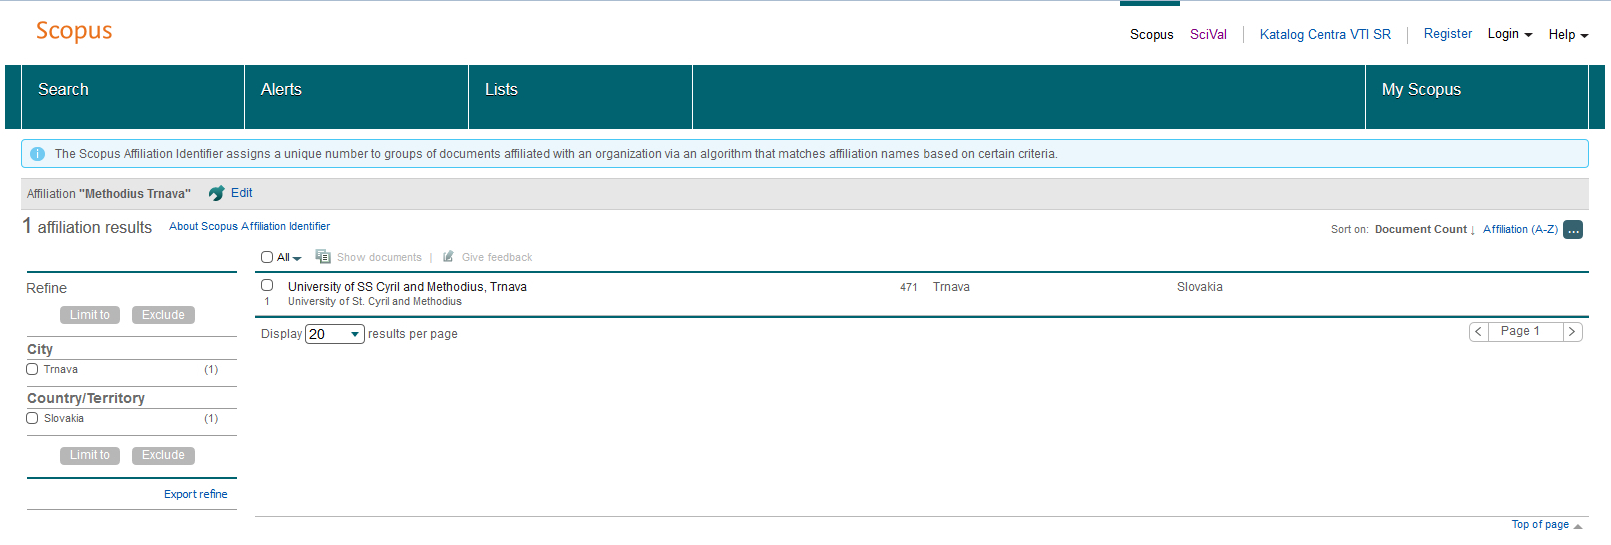
\includegraphics[width=\textwidth]{obr/scopus02-cut.jpg}
  \caption{Scopus -- zoznam inštitúcií.}
  \label{fig:scopus.institutionlist}
\end{figure}

\begin{figure}
  \centering
  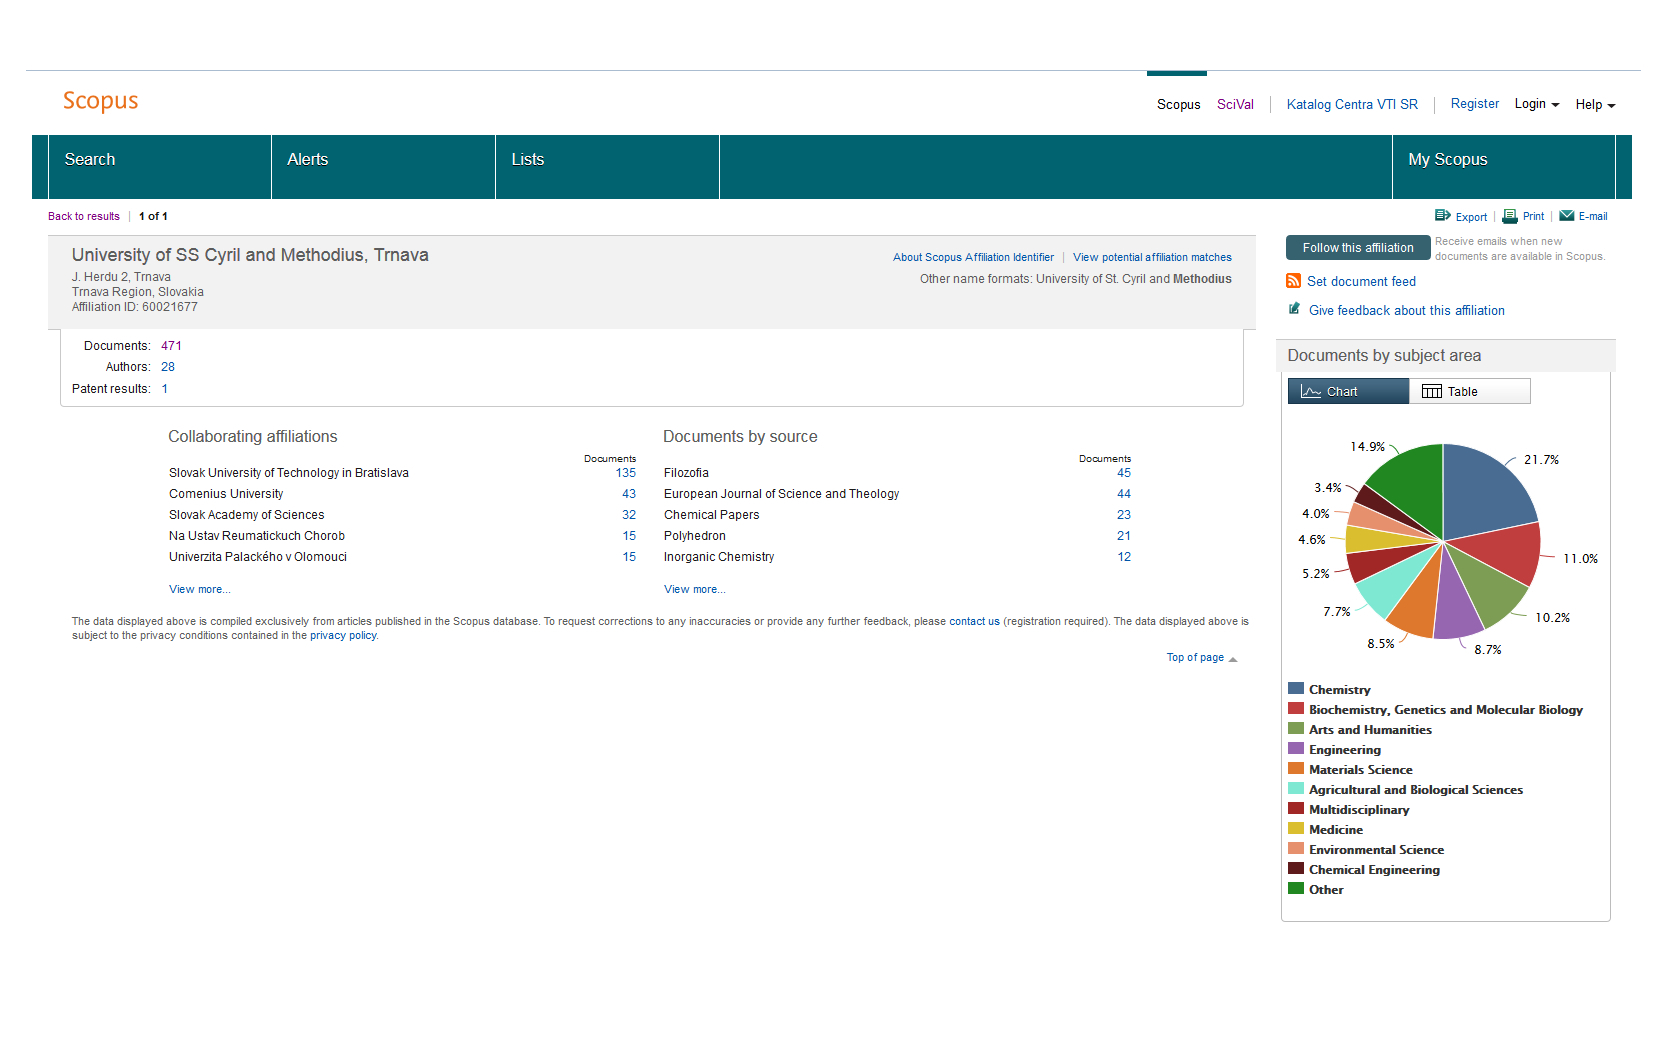
\includegraphics[width=\textwidth]{obr/scopus03-cut.jpg}
  \caption{Scopus -- informácie o inštitúcii.}
  \label{fig:scopus.institutioninfo}
\end{figure}

Kliknutím na položku sa zobrazí stránka s bližšími informáciami
(Obr.\,\ref{fig:scopus.institutioninfo}), ako sú adresa, celkový počet
dokumentov: 471, celkový počet autorov: 28, zoznam spoluautorských inštitúcii,
zoznam časopisov, v ktorých boli publikované práce a koláčový graf rozdelenia
záznamov na vedecké oblasti podľa Scopus-u.

Kliknutím na číslo 471 (počet záznamov dokumentov) sa zobrazí stránka so
zoznamom dokumentov ako ukazuje Obr.\,\ref{fig:scopus.documentlist}.

\begin{figure}
  \centering
  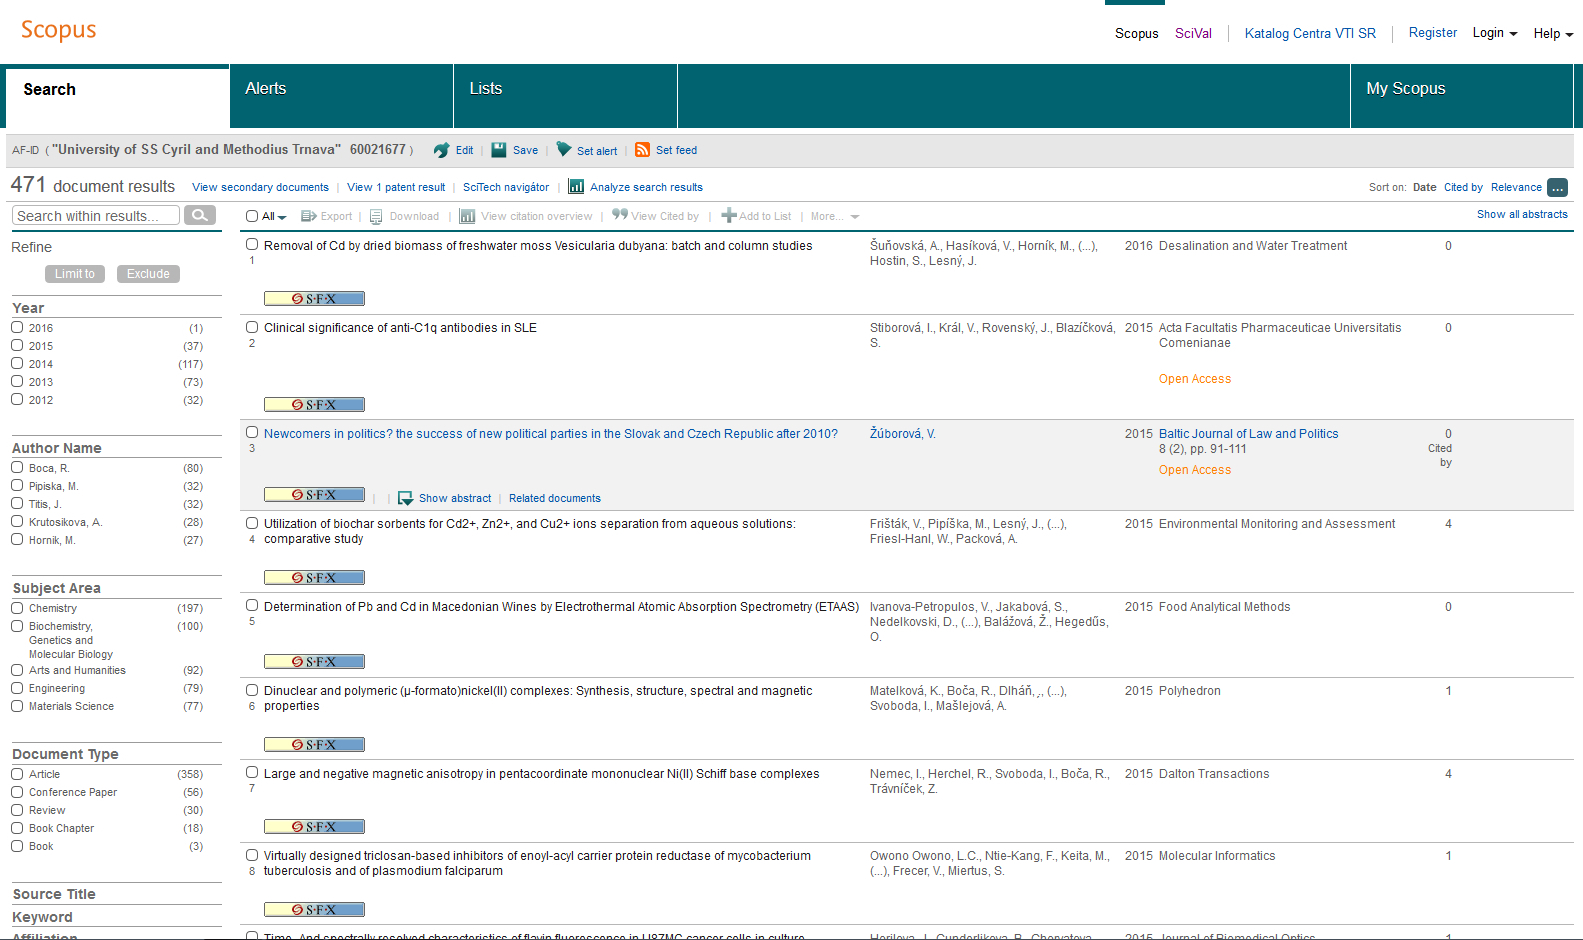
\includegraphics[width=\textwidth]{obr/scopus04-cut.jpg}
  \caption{Scopus -- zoznam dokumentov.}
  \label{fig:scopus.documentlist}
\end{figure}

Keďže nástroje Scopusu neumožňujú vyhľadávať podľa fakulty, alebo dokonca
katedry (\emph{department}), bibliografické záznamy Fakulty prírodných vied sme
získali filtrovaním samotných záznamov. Z počiatku sme vylúčili vedecké oblasti
(\emph{Subject Area}), ktoré nesúvisia s činnosťou FPV UCM:
\begin{itemize}

\item \emph{Art and Humanites:} umenie a humanitné vedy,

\item \emph{Social Sciences:} sociálne vedy,

\item \emph{Business, Management and Accounting:} biznis, manažment a
  účtovníctvo,

\item \emph{Psychology:} psychológia,

\end{itemize}
a publikácie z roku 1991, pretože v tomto roku UCM ešte nebola založená. Počet
záznamov sa znížil na 356.

Ďalším krokom bolo vylúčenie článkov, ktorých autori nepôsobia v rámci Fakulty
prírodných vied podľa Tab.\,\ref{tab:scopus.exauthors}.  Počet záznamov sa
tak znížil na 329.

\begin{table}
\centering\small
\begin{tabular}{lccc}
  \hline\noalign{\vspace{.3ex}}
  Meno autora                & Afiliácia \\[0.3ex]
  \hline\noalign{\vspace{.5ex}}
  Bezáková, Zuzana           & -- \\
  Ferriero, Giorgio          & -- \\
  Halenár, Robert            & -- \\
  Jačala, Jozef              & -- \\
  Mura, Ladislav             & -- \\[1ex]
  Nováková, Renata           & -- \\
  Rovenský, Jozef            & -- \\
  Rovenský, Jozef A.         & -- \\
  Trnka, Andrej              & -- \\
  Vicente, Romana Albaladejo & -- \\[0.5ex]
  \hline
\end{tabular}
\caption{Scopus -- vylúčení autori.}
\label{tab:scopus.exauthors}
\end{table}

Vytriedené záznamy sme uložili do formátu .csv na scientometrickú analýzu pomocou Export $\rightarrow$ CSV (Excel), Citation Information Only (iba citácie) ako je ukázané na Obr.\,\ref{fig:scopus.export}.

\begin{figure}
  \centering
  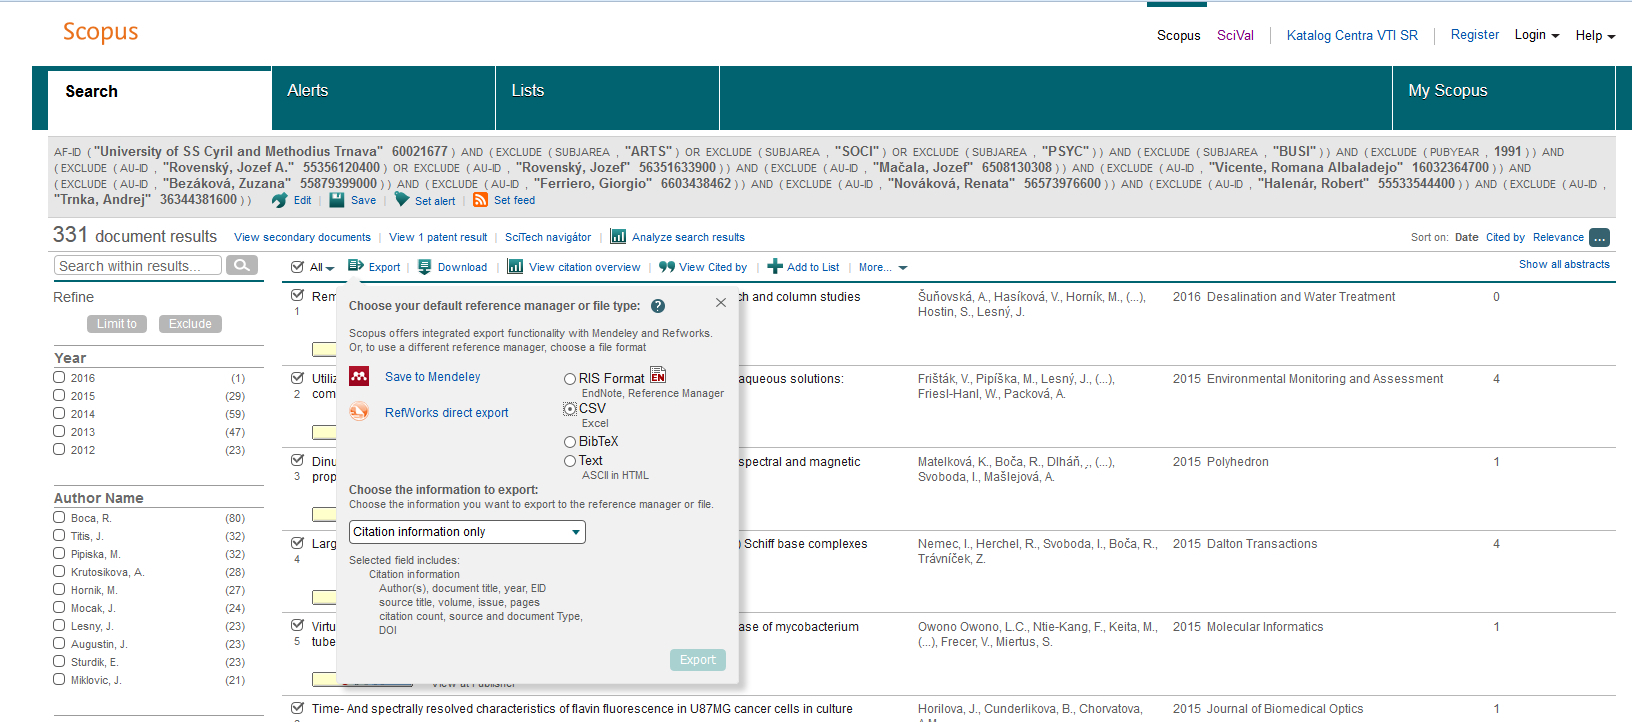
\includegraphics[width=\textwidth]{obr/scopus10-cut.jpg}
  \caption{Scopus -- export dát do súboru.}
  \label{fig:scopus.export}
\end{figure}


\subsection{Citačná databáza Web of Science}

Do citačného registra \emph{Thomson Reuters Web of Science} sme pristupovali cez
portál \emph{Centra Vedecko-Technických Informácií
  SR}\footnote{\url{http://www.cvtisr.sk}}. Citačné záznamy sme získali zo
stránok Web of Science\footnote{\url{https://ezproxy.cvtisr.sk:2774/}}
(17.\,5.\,2016). Pretože vyhľadávací systém webového rozhrania neumožňuje
vyhľadávať konkrétnu inštitúciu ako to je v prípade Scopus-u, hľadali sme podľa
adresy (ADRESS) \uv{Trnava} a \uv{Methodius*} (pre vyňatie publikácií Trnavskej
Univerzity v Trnave) ako ukazujú obrázky \ref{fig:wos.search} a
\ref{fig:wos.documentlist}.

\begin{figure}
  \centering
  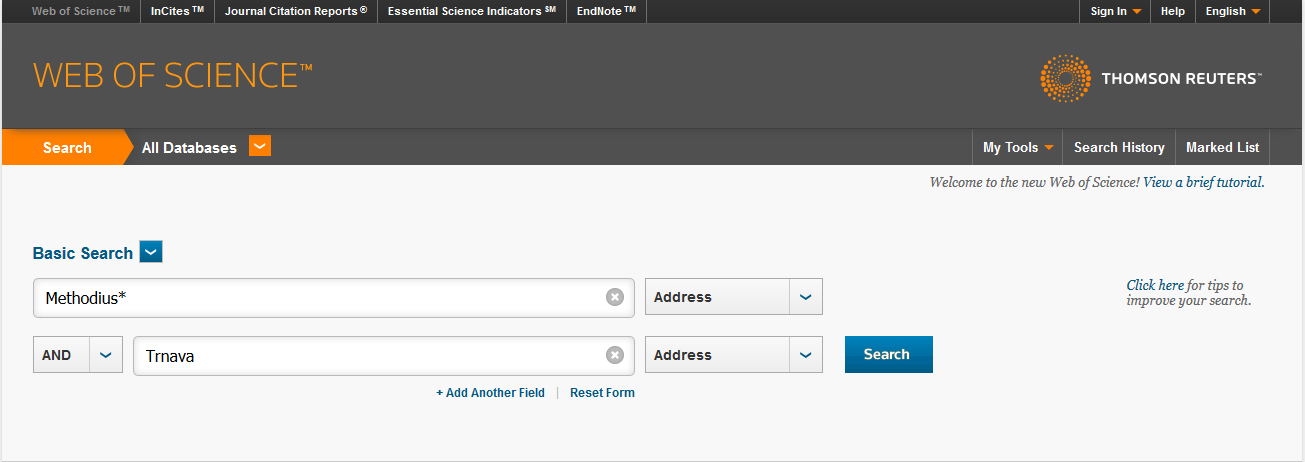
\includegraphics[width=\textwidth]{obr/wos01-cut.jpg}
  \caption{WoS -- vyhľadávanie záznamov.}
  \label{fig:wos.search}
\end{figure}

\begin{figure}
  \centering
  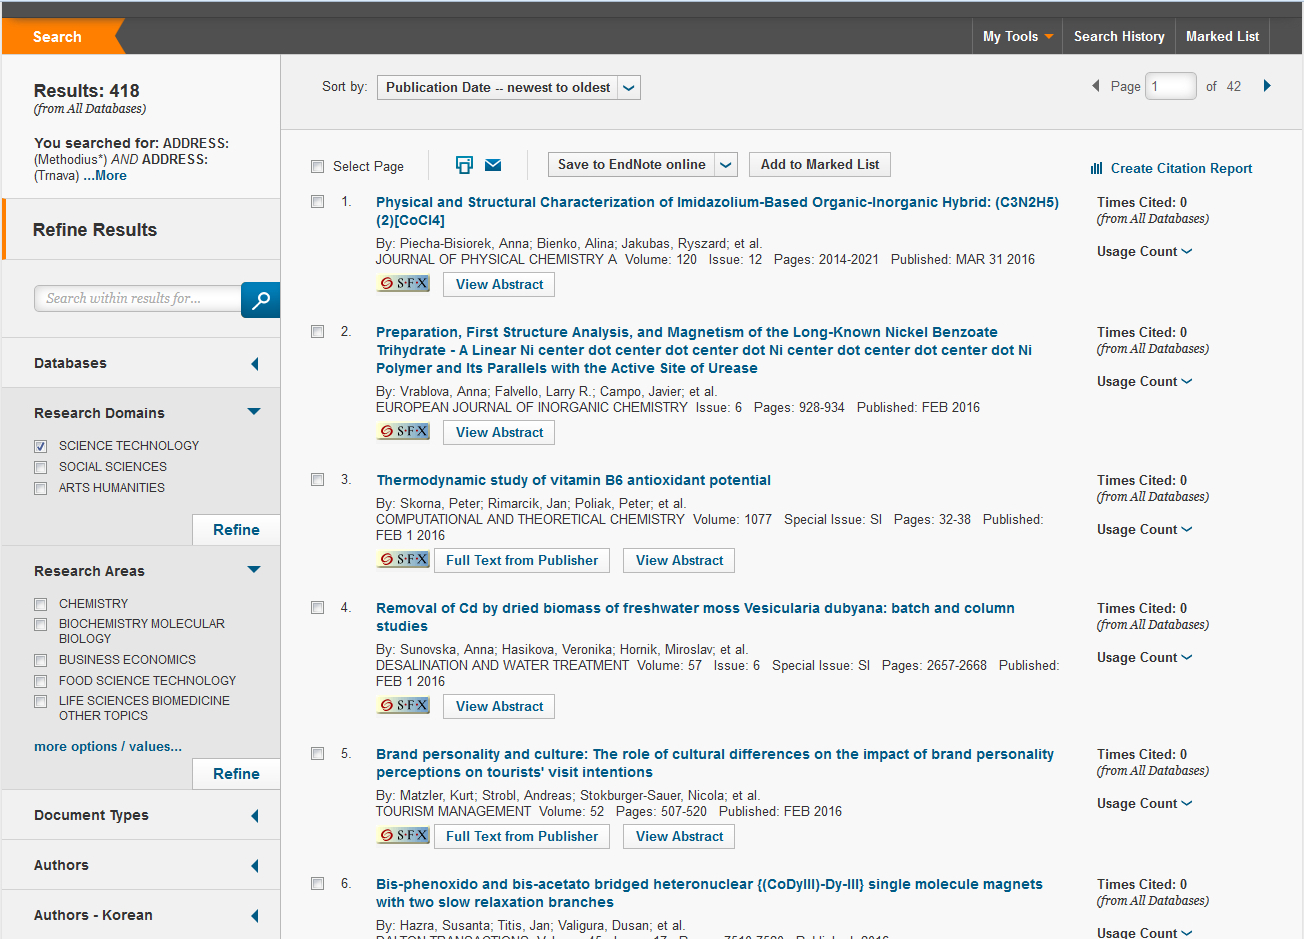
\includegraphics[width=\textwidth]{obr/wos02-cut.jpg}
  \caption{WoS -- zoznam dokumentov, ktoré sú výsledkom vyhľadávania z Obr\,\ref{fig:wos.search}.}
  \label{fig:wos.documentlist}
\end{figure}

Filtrovanie výsledkov do domény vedy a techniky (SCIENCE AND TECHNOLOGY) znížilo
počet záznamov na 318. Odstránenie záznamov z vedeckých oblastí (Research
Areas): Sociológia (SOCIOLOGY), Iné sociálne vedy (SOCIAL SCIENCES OTHER TOPICS)
a biznisu (BUSINESS ECONOMICS) ukazuje Obr.\,\ref{fig:wos.areaselection}. Na
koniec sme definovali krajinu (Countries/Territories) ako Slovensko (SLOVAKIA),
čo nám dalo konečný počet záznamov 293.

\begin{figure}
  \centering
  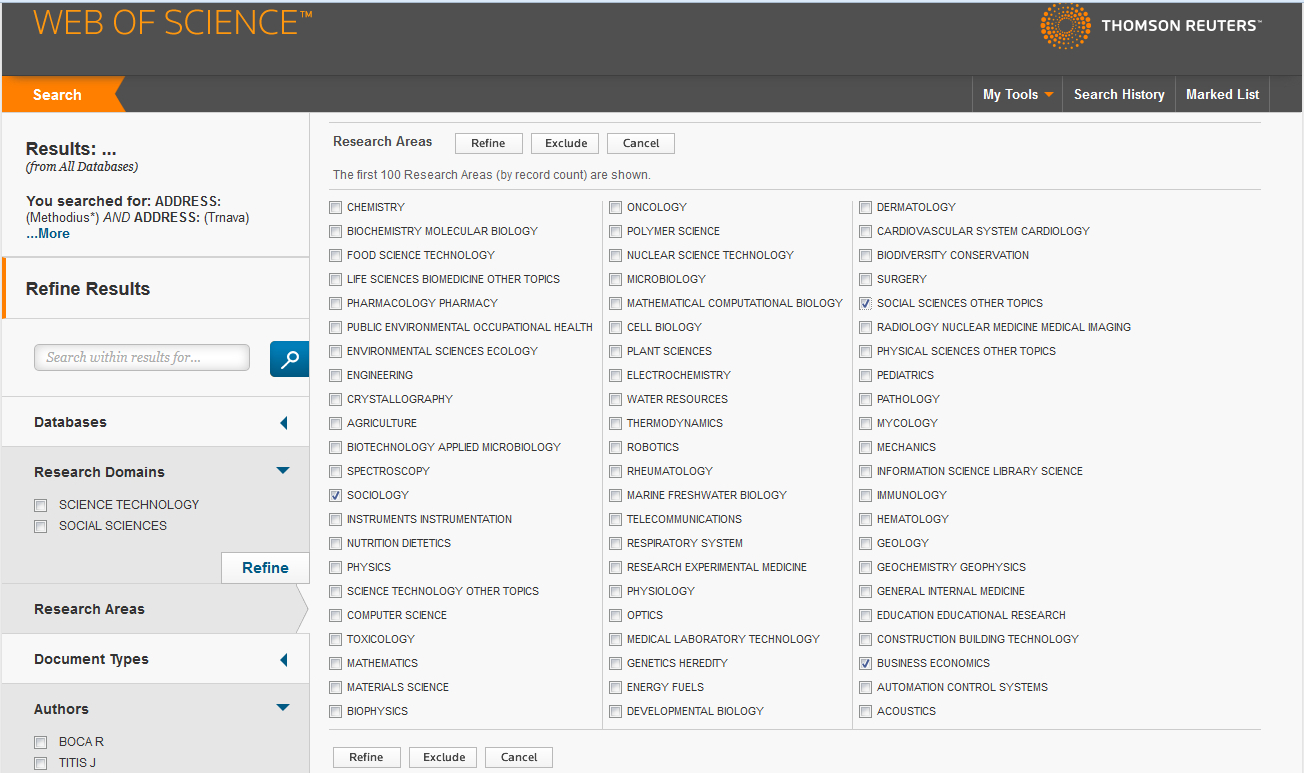
\includegraphics[width=\textwidth]{obr/wos04-cut.jpg}
  \caption{WoS -- výber vedeckých oblastí.}
  \label{fig:wos.areaselection}
\end{figure}

\begin{figure}
  \centering
  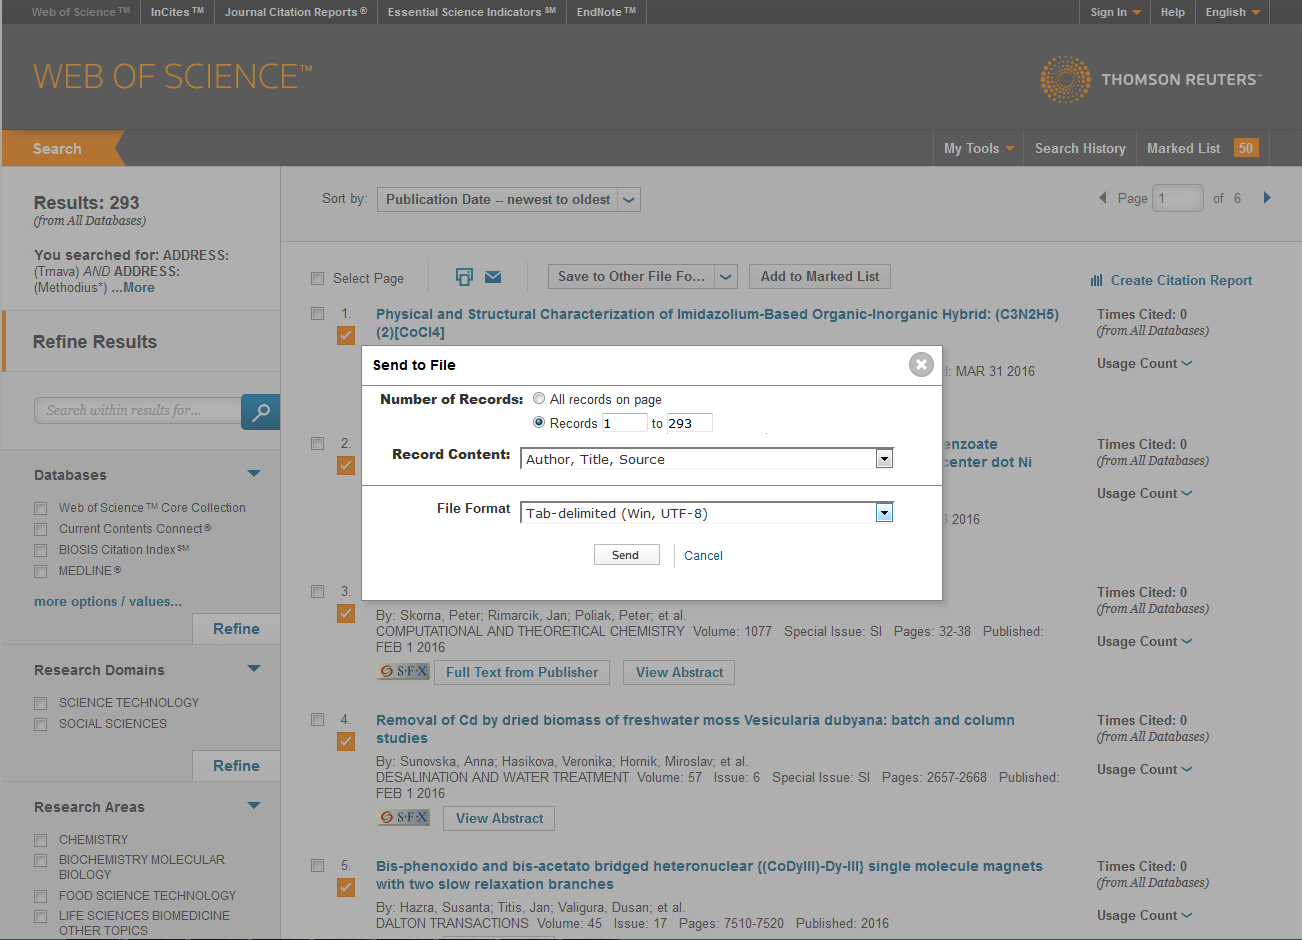
\includegraphics[width=\textwidth]{obr/wos06-cut.jpg}
  \caption{WoS -- export dát do súboru.}
  \label{fig:wos.export}
\end{figure}

Obr.\,\ref{fig:wos.export} zobrazuje ako sme tieto záznamy pomocou funkcie „save
to other formats“ uložili do csv súboru. Pre uloženie všetkých záznamov je
potrebné zvoliť rozsah (1 to 293) a formát (\emph{Author}, \emph{Title},
\emph{Source}).


\section{Spracovanie bibliometrických dát}

Síce webové rozhrania \emph{Scopus} a \emph{WoS} poskytujú základné
scientometrické nástroje ako napr. výpočet $h$-indexu, ale možnosti dodatočného
triedenia (ako napr. zatriedenie do jednotlivých katedier) sú obmedzené. Taktiež
neumožňuje použiť modernejšie citačné indexy (viď kapitolu
\ref{sec:citation.indicators}). Preto sme sa rozhodli použiť program Publish or
Perish\footnote{\url{http://www.harzing.com/resources/publish-or-perish}}.


\subsection{Dodatočné spracovanie stiahnutých záznamov}

Ako vstup sme použAko vstup sme použili csv súbory exportované z databáz
\emph{Scopus} a \emph{WoS} (označené ako \uv{\texttt{scopus~17.5.2016.csv}} a
\uv{\texttt{WoS~17.5.2016.csv}}). V textovom súbore
\uv{\texttt{scopus~17.5.2016.csv}} sme zmazali duplicitné záznamy a opravili
chybný zápis mien podľa tabuľky \ref{tab:wos.namecorrections}.

\begin{table}
\centering\small
\begin{tabular}{ll}
  \hline\noalign{\vspace{.3ex}}
  Pôvodné meno & Opravené meno \\[0.3ex]
  \hline\noalign{\vspace{.5ex}}
  Boa          & Boča       \\
  Boça         & Boča       \\
  Horváthovái  & Horváthová \\
  Oturdík      & Šturdík    \\
  Titiş        & Titiš      \\[0.5ex]
  \hline
\end{tabular}
\caption{Oprava chýb v menách autorov v súbore \uv{\texttt{scopus~17.5.2016.csv}}.}
\label{tab:wos.namecorrections}
\end{table}

Pretože databáza \emph{Scopus} nám umožnila odstrániť všetky záznamy z iných
fakúlt, súbor \uv{\texttt{scopus~17.5.2016.csv}} sme ďalej neupravovali a
konečný počet bibliografických záznamov je 324.

\begin{table}
\centering\small
\begin{tabular}{lc}
  \hline\noalign{\vspace{.3ex}}
  Meno            & Fakulta \\[0.3ex]
  \hline\noalign{\vspace{.5ex}}
  Balaz           & -- \\
  Balazova        & -- \\
  Bezakova        & -- \\
  Lukac           & -- \\
  Rovensky        & -- \\[1ex]
  Jurinova        & -- \\
  Ferriero        & -- \\
  Trnka           & -- \\
  Halenar         & -- \\
  Mura            & -- \\[1ex]
  Novakova Renata & -- \\[0.5ex]
  \hline
\end{tabular}
\caption{Mená pracovníkov, ktorí nepatria do Fakulty prírodných vied.}
\label{tab:wos.excludedstaff}
\end{table}

\emph{Web of Science} má veľmi obmedzené možnosti triedenia väčšieho množstva
dát, napr. je možné filtrovať podľa 100 autorov (Scopus tákéto obmedzenie
nepozná). Z týchto dôvodov sme súbor \uv{\texttt{WoS~17.5.2016.csv}} spracovali
dodatočne. Odstránili sme záznamy s menami podľa tabuľky
\ref{tab:wos.excludedstaff} a získali sme 288 záznamov.


\subsection{Rozdelenie dát do katedier}

Stiahnuté bibliografické záznamy sme rozdelili do ôsmych súborov
(tab.\,\ref{tab:staffsort}) podľa pracovníkov, ktorí pôsobia (prípadne pôsobili)
v rámci danej katedry. Súbory zo Scopusu a WoS sme spracovali samostatne,
pretože zo získaných dát nie je možné dohľadať indentické citácie. Niektoré mená
autorov zo Scopusu a všetky z WoS sú písané bez diakritiky. Práce, ktoré vznikli
ako spolupráca ľudí z viacerých katedier sú zaradené iba do jednej z katedier
(podľa kľúčových slov).Záznamy Katedry biofyziky a Katedry odbornej jazykovej
prípravy boli z analýzy vyňaté zahrnuté pre veľmi nízky počet dát.

\begin{table}
\centering\small
\begin{tabular}{lllll}
  \hline\noalign{\vspace{.3ex}}
  Katedra  & Katedra        & Katedra & Katedra         & Katedry      \\
  biológie & biotechnológii & chémie  & ekochémie       & aplikovanej  \\ 
           &                &         & a~rádioekológie & informatiky  \\ 
           &                &         &                 & a~matematiky \\[0.3ex]
  \hline\noalign{\vspace{.5ex}}
  Janeček, Štefan, Š. & Breierová      & Baran       & Babulicová & Ďurikovič   \\
  Godány              & Faragó         & Bednárová   & Fargašová  & Gudába      \\
  Preťová             & Gazdík         & Beinrohr    & Horník     & Hostovecký  \\
  Siekel              & Havrlentová    & Boča        & Lesný      & Huraj       \\
  Ürgeová             & Chraštieľ      & Boronová    & Pipíška    & Kostolanský \\[1ex]
  Vidová              & Kováčik        & Gašparová   & Uhrovčík   &             \\
                      & Kraic, Ján, J. & Halgaš      &            &             \\
                      & Maliar         & Jóna        &            &             \\
                      & Miertuš        & Krutošíková &            &             \\
                      & Ondrejovič     & Kružlicová  &            &             \\[1ex]
                      & Šturdík        & Kováčiková  &            &             \\
                      & Urban          & Lehotay     &            &             \\
                      &                & Miklovič    &            &             \\
                      &                & Močák       &            &             \\
                      &                & Nemeček     &            &             \\[1ex]
                      &                & Rabara      &            &             \\
                      &                & Rimančík    &            &             \\
                      &                & Titiš       &            &             \\[0.5ex]
  \hline
\end{tabular}
\caption{Rozdelenie pracovníkov do jednotlivých katedier.}
\label{tab:staffsort}
\end{table}


\subsection{Scientometrická analýza dát}

Pomocou programu \emph{Publish or Perish} (Harzing, 2010) sme vypočítali citačné
indexy pre jednotlivé súbory dát (zobrazené na Obr. \ref{fig:pop.departmentfiles}).

\begin{figure}
  \centering
  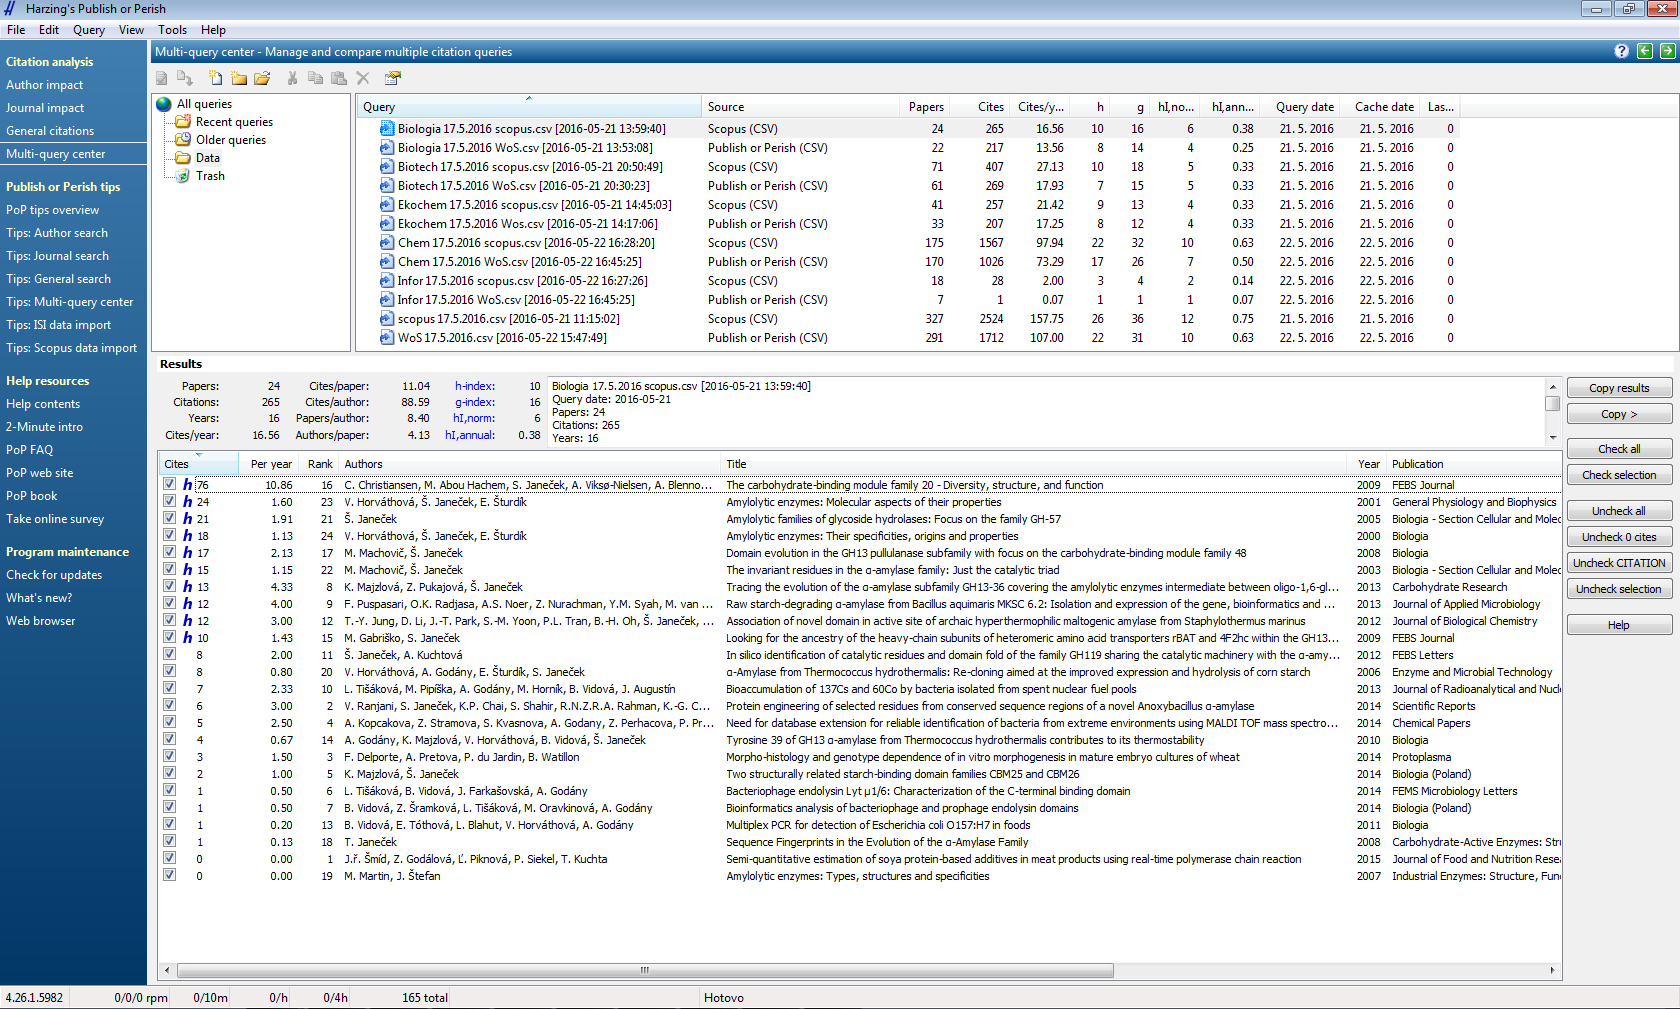
\includegraphics[width=\textwidth]{obr/publish-or-perish.jpg}
  \caption{Súbory dát jednotlivých katedier v programe \emph{Publish or Perish}.}
  \label{fig:pop.departmentfiles}
\end{figure}

V tabuľkovom kalkulátore sme zhotovili grafické zobrazenie vývoja publikačnej činnosti
(a citovanosti) jednotlivých katedier v čase.

%%% Local Variables:
%%% TeX-master: "diplomovka"
%%% End:
